\documentclass[10pt]{article}
\usepackage[polish]{babel}
\usepackage[utf8]{inputenc}
\usepackage[T1]{fontenc}
\usepackage{amsmath}
\usepackage{amsfonts}
\usepackage{amssymb}
\usepackage[version=4]{mhchem}
\usepackage{stmaryrd}
\usepackage{graphicx}
\usepackage[export]{adjustbox}
\graphicspath{ {./images/} }

\title{50 D) \(\begin{gathered}\text { Akademia } \\ \text { Pomorska } \\ \text { w Stupsku }\end{gathered}\) }

\author{}
\date{}


\begin{document}
\maketitle
\begin{center}
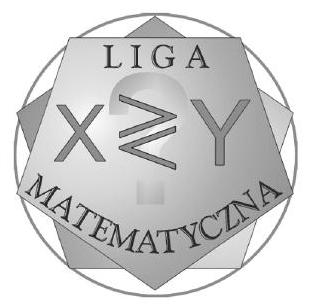
\includegraphics[max width=\textwidth]{2024_11_21_943a59a868dc10504530g-1}
\end{center}

LIGA MATEMATYCZNA\\
im. Zdzisława Matuskiego\\
PÓŁFINAŁ 26 lutego 2019\\
GIMNAZJUM\\
(klasa VII i VIII szkoły podstawowej, klasa III gimnazjum)

\section*{ZADANIE 1.}
W rombie \(A B C D\) punkty \(M\) i \(N\), różne od punktów \(A, B\) i \(C\), leżą na odcinkach odpowiednio \(A B, B C\) tak, że trójkąt \(D M N\) jest równoboczny oraz \(|A D|=|M D|\). Wyznacz miarę kąta \(A B C\).

\section*{ZADANIE 2.}
Znajdź wszystkie liczby trzycyfrowe, które są 11 razy większe od sumy swoich cyfr.

\section*{ZADANIE 3.}
Wyznacz wszystkie pary \((x, y)\) liczb całkowitych dodatnich spełniające warunki \(x+y=320\) \(\operatorname{oraz} \operatorname{NWD}\{x, y\}=40\).

\section*{ZADANIE 4.}
Bartek wybrał pewną liczbę (niekoniecznie różnych) liczb ze zbioru \(\{-1,0,1,2\}\) w taki sposób, że ich suma jest równa 19, a suma ich kwadratón jest równa 99. Jaka jest największa możliwa wartość sumy sześcianów liczb wybranych przez Bartka?

\section*{ZADANIE 5.}
Sześciokąt, którego wszystkie kąty mają miarę \(120^{\circ}\) wpisano w trójkąt równoboczny o boku o długości 9. Długości trzech boków sześciokąta są równe 5, 5, 3. Oblicz obwód sześciokąta.\\
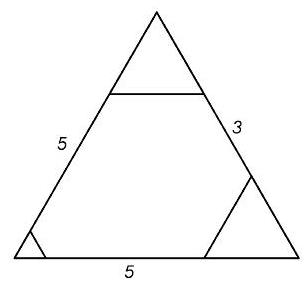
\includegraphics[max width=\textwidth, center]{2024_11_21_943a59a868dc10504530g-1(1)}


\end{document}